\documentclass[a4paper]{article}
\usepackage[T1]{fontenc}
\usepackage[utf8]{inputenc}
\usepackage{graphicx,tocloft,siunitx,amssymb,amsmath,float,subcaption,ragged2e}\usepackage[american]{circuitikz}
%\usepackage{subcaption,pgf,pgfplots}
\usepackage[top=3cm,left=3cm,right=3cm]{geometry}
\graphicspath{{img/}}
\renewcommand\cftsecfont{\normalfont}
\renewcommand\cftsecpagefont{\normalfont}
\renewcommand{\cftsecleader}{\cftdotfill{\cftsecdotsep}}
\renewcommand\cftsecdotsep{\cftdot}
\renewcommand\cftsubsecdotsep{\cftdot}
\renewcommand\cftsubsubsecdotsep{\cftdot}
\title{Lab 3:Kirchhoff's Laws}
\author{
    Sebastián Nava López\\
    \and
    Ericka Sabrina Pensamiento R.\\
    \and
    Salvador Palos Gil
}
%\captionsetup[subfigure]{justification=raggedright}
\begin{document}
\begin{titlepage}
    \centering
    {\Huge Instituto Politécnico Nacional}\\[3ex]
    {\huge Escuela Superior de Cómputo}\\[8ex]
    {\huge Fundamental Circuit Analysis}\\[12ex]
    {\Large Lab 3:Kirchhoff's Laws}\\[20ex]
    {\Large Group: 1CV7 Team: 7 \\[8ex]
    Sebastian Nava López\\[4ex]
    Sabrina Erika Pensamiento Robledo\\[4ex]
    Salvador Palos Gil\\[18ex]
    }
    \large{Elaboration: March 13,2018\hspace{8em} Due date: March 20,2018}
\end{titlepage}
\tableofcontents
\newpage
\section{Introduction}
Although Ohm’s law is useful to be able to reduce series and parallel resistors in a circuit when they occur, circuits in general are not composed exclusively of such combinations. Although in our analysis we will always assume that the elements are linear and are thus described by a straight-line characteristic that passes through the origin, it is important to realize that some very useful and practical elements do exist that exhibit a nonlinear resistance characteristic; that is, the voltage–current relationship is not a straight line. For such cases there are a powerful set of relations called Kirchhoff's laws which enables the engineer to analyze arbitrary circuits. There are two laws:
\begin{itemize}
\item The first law or the \textit{junction} rule: \textit{for a given junction or node in a circuit, the sum of the currents entering equals the sum of the currents leaving}.This law is a statement of charge conservation. Once again it must be emphasized that the latter statement means that the sum of the variables that have been defined entering the node is equal to the sum of the variables that have been defined leaving the node, not the actual currents. Recall that current is charge in motion. Based on our background in physics, charges cannot be stored at a node. In other words, if we have a number of charges entering a node, then an equal number must be leaving that same node.

\item The second law or the \textit{loop rule}: \textit{around any closed loop in a circuit, the sum of the potential differences across all elements is zero.} This law is a statement of energy conservation, in that any charge that starts and ends up at the same point with the same velocity must have gained as much energy as it lost.
\end{itemize}
Finally, it is possible to generalize Kirchhoff's current law to include a closed surface. By a closed surface we mean some set of elements completely contained within the surface that are interconnected. Since the current entering each element within the surface is equal to that leaving the element (i.e., the element stores no net charge), it follows that the current entering an interconnection of elements is equal to that leaving the interconnection. Therefore, Kirchhoff's current law can also be stated as follows: The algebraic sum of the currents entering any closed surface is zero
Kirchhoff's Laws for current and voltage lie at the heart of circuit analysis. With these two laws, plus the equations for individual component (resistor, capacitor, inductor), we have the basic tool set we need to start analyzing circuits. To really understand all of this, it is essential to understand concepts like: 
 
\begin{itemize}
{\item \textbf{Circuit}: Which comes from the word circle. It is a collection of real components, power sources, and signal sources, all connected so current can flow in a complete circle
\begin{itemize}
\item \textbf{Closed circuit}: A circuit is closed if the circle is complete, if all currents have a path back to where they came from.
\item \textbf{Open circuit}: A circuit is open if the circle is not complete, if there is a gap or opening in the path.
\item \textbf{Short circuit}: A short happens when a path of low resistance is connected (usually by mistake) to a component. The resistor shown below is the intended path for current, and the curved wire going around it is the short. Current is diverted away from its intended path, sometimes with damaging results. The wire shorts out the resistor by providing a low-resistance path for current (probably not what the designer intended).
\item \textbf{Make or break}: You make a circuit by closing the current path, such as when you close a switch. Breaking a circuit is the opposite. Opening a switch breaks the circuit.
\end{itemize}}
\item \textbf{Branches}: Are the connections between nodes. A branch is an element (resistor, capacitor, source, etc.). The number of branches in a circuit is equal to the number of elements.
{\item \textbf{Loops}: Are any closed path going through circuit elements. To draw a loop, select any node as a starting point and draw a path through elements and nodes until the path comes back to the node where you started. There is only one rule, a loop can visit (pass through) a node only one time. It is right if loops overlap or contain other loops
\begin{itemize}
\item \textbf{Mesh}: A mesh is a loop that has no other loops inside it. You can think of this as one mesh for each "open window" of a circuit.
\end{itemize}}
{\item \textbf{Reference node}: During circuit analysis we usually pick one of the nodes in the circuit to be the reference node. Voltages at other nodes are measured relative to the reference node. Any node can be the reference, but two common choices that simplify circuit analysis are:
\begin{itemize}
\item The negative terminal of the voltage or current source powering the circuit.
\item Or, the node connected to the greatest number of branches
\end{itemize}}
\end{itemize}
After clarifying all these concepts, we are ready to jump right into circuit analysis and solving problems.
Kirchhoff's laws were named like that because Gustav Kirchhoff was responsible for the creation of the already mentioned laws. These were understood as an extension from the energy conservation law and are based on Georg Simon Ohm's theory. This, however, was not Kirchhoff's only contribution to science. After becoming a physics teacher in the University of Heidelberg, with Robert Bunsen's collaboration, discovered cesium (1860) and rubidium (1861). Years later, he successfully explained why there were numerous black lines that appeared in the solar spectrum, known as Fraunhofer lines.

\newpage
\section{Development}
%----------Circuit1
\subsection{Verification of Kirchhoff's Voltage Law}
\subsubsection{Calculations}
In the first part, we wire the components in series as showed in the diagram:
%----------Circut 1 Diagram
\begin{minipage}{.7\textwidth}
  \begin{circuitikz}
		\draw (0,3) to [R=$R_1$,*-*] (3,3)
    	to [V=$V_{S1}$,-*] (5,3)
    	to [R=$R_2$] (7,3) -- (8,3)
    	to [R=$R_3$,*-] (8,0) to [short,-*] (4,0) -- (0,0)
    	(0,3) to [V=$V_{S1}$] (0,0)
    	{[anchor=south east](0,3) node {A}
    	[anchor=south east](3,3) node {B} 
    	[anchor=south east](5,3) node {C}
    	[anchor=south west](8,3) node {D}
		[anchor=north west](4,0) node {0}};
    \end{circuitikz}
\end{minipage}\raggedright
\begin{minipage}{.3\textwidth}
    \begin{tabular}{|c|c|c|}\hline
        Element & Value & Power Rat.\\\hline
        $V_{S1}$ & $\SI{9}{\volt}$ & $0$\\\hline
        $V_{S2}$ & $\SI{5}{\volt}$ & $0$\\\hline
        $R_1$ & $\SI{470}{\ohm}$ & $\SI{1/2}{\volt}$\\\hline
        $R_2$ & $\SI{330}{\ohm}$ & $\SI{1/2}{\volt}$\\\hline
        $R_3$ & $\SI{560}{\ohm}$ & $\SI{1/2}{\volt}$\\\hline
    \end{tabular}
\end{minipage}
Then, applying Kirchhoff's Voltage Law, we have that:
\begin{gather*}
    -V_{si}+VR_1+V_{s2}+VR_2+VR_3=0\\
    -9+470I+5+330I+56I=0\\
    1360I=9-5\\
    I=\frac{4}{1360}\si{\ampere}\qquad I=\SI{2.941}{\milli\ampere}
\end{gather*}
Now that we have the current value we can calculate the voltage value for each segment in the
circuit.\\
For $V_{0A}$:
\begin{align*}
    V_{0A}&=-V_{S1}\\
    V_{0A}&=-9V
\end{align*}
For $V_{AB}$:
\begin{align*}
    V_{AB}&=VR_1\\
    V_{AB}&=IR_1\\
    V_{AB}&=(\SI{2.941}{\milli\ampere})(\SI{470}{\ohm})\\
    V_{AB}&=\SI{1.382}{\volt}
\end{align*}
For $V_{BC}$:
\begin{align*}
    V_{BC}&=V_{S2}\\
    V_{BC}&=5V
\end{align*}
For $V_{CD}$:
\begin{align*}
    V_{CD}&=VR_2\\
    V_{CD}&=IR_2\\
    V_{CD}&=(\SI{2.941}{\milli\ampere})(\SI{330}{\ohm})\\
    V_{CD}&=\SI{0.970}{\volt}
\end{align*}
For $V_{D0}$:
\begin{align*}
    V_{D0}&=VR_3\\
    V_{D0}&=IR_1\\
    V_{D0}&=(\SI{2.941}{\milli\ampere})(\SI{560}{\ohm})\\
    V_{D0}&=\SI{1.647}{\volt}
\end{align*}
Finally, the sum of all voltages is:
\begin{align*}
    \sum\nolimits_{V}&=V_{0A}+V_{AB}+V_{BC}+V_{CD}+V_{D0}\\
    \sum\nolimits_{V}&=-\SI{9}{\milli\watt}+\SI{1.382}{\milli\watt}+\SI{5}{\milli\watt}+\SI{0.970}{\milli\watt}+\SI{1.647}{\milli\watt}\\
    \sum\nolimits_{V}&=\SI{-2.4e-4}{\milli\watt}\qquad
    \therefore\sum\nolimits_{V}\approx 0\si{\volt}
\end{align*}
Then, Power(P) is given by:
\[P=IV\]
Power $P_{0A}$ is equal to:
\begin{align*}
    P_{0A}&=IV_{0A}\\
    P_{0A}&=(\SI{2.941}{\milli\ampere})(\SI{-9}{\volt})\\
    P_{0A}&=\SI{-26.469}{\milli\watt}\\
\end{align*}
For $P_{AB}$:
\begin{align*}
    P_{AB}&=IV_{AB}\\
    P_{AB}&=(\SI{2.941}{\milli\ampere})(\SI{1.382}{\volt})\\
    P_{AB}&=\SI{4.064}{\milli\watt}\\
\end{align*}
For $P_{BC}$:
\begin{align*}
    P_{BC}&=IV_{BC}\\
    P_{BC}&=(\SI{2.941}{\milli\ampere})(\SI{5}{\volt})\\
    P_{BC}&=\SI{14.705}{\milli\watt}\\
\end{align*}
For $P_{CD}$:
\begin{align*}
    P_{CD}&=IV_{CD}\\
    P_{CD}&=(\SI{2.941}{\milli\ampere})(\SI{0.970}{\volt})\\
    P_{CD}&=\SI{2.853}{\milli\watt}\\
\end{align*}
For $P_{D0}$:
\begin{align*}
    P_{D0}&=IV_{D0}\\
    P_{D0}&=(\SI{2.941}{\milli\ampere})(\SI{1.647}{\volt})\\
    P_{D0}&=\SI{4.844}{\milli\watt}\\
\end{align*}
The sum of all the powers is:
\begin{align*}
    \sum\nolimits_{P}&=P_{0A}+P_{AB}+P_{BC}+P_{CD}+P_{D0}\\
    \sum\nolimits_{P}&=-\SI{-26.469}{\volt}+\SI{1.382}{\volt}+\SI{5}{\volt}+\SI{0.970}{\volt}+\SI{1.647}{\volt}\\
    \sum\nolimits_{P}&=\SI{-2.941e-6}{\volt}\qquad
    \therefore\sum\nolimits_{P}\approx \SI{0}{\watt}
\end{align*}
\subsubsection{Measurements}
Measured Current($I$) :$\SI{2.88}{\milli\ampere}$
\begin{table}[H]
    \centering
    \resizebox{\textwidth}{!}{
\begin{tabular}{|c|c|c|c|c|c|}\hline
    Measurements & Theoretical & Measured & Theoretical & Measured &
    Absorb(A)/\\
     &  Value (\si{\volt}) &  Value (\si{\volt}) & Power (\si{\milli\watt}) & Power (\si{\milli\watt}) & Supply(S)\\\hline
     Voltage $V_{0A}$ & -9.000 & -9.000 & -26.469 & -25.900 & S\\\hline
     Voltage $V_{AB}$ & 1.382 & 1.220 & 4.064 & 3.510 & A\\\hline
     Voltage $V_{BC}$ & 5.000 & 5.250 & 14.705 & 15.120 & A\\\hline
     Voltage $V_{CD}$ & 0.970 & 0.910 & 2.853 & 2.600 & A\\\hline
     Voltage $V_{D0}$ & 1.647 & 1.550 & 4.844 & 4.460 & A\\\hline
      & $\sum_V=\SI{-2.941}{\micro\volt}$ & $\sum_V=\SI{-0.070}{\milli\volt}$ &
      $\sum_P=\SI{-3.000}{\micro\watt}$ & $\sum_P=\SI{-0.210}{\micro\watt}$ & \\\hline
\end{tabular}}
\caption{Theoretical and experimental voltage values}\label{table:1}
\end{table}
\subsubsection{Simulation}
\begin{figure}[H]
    \centering
    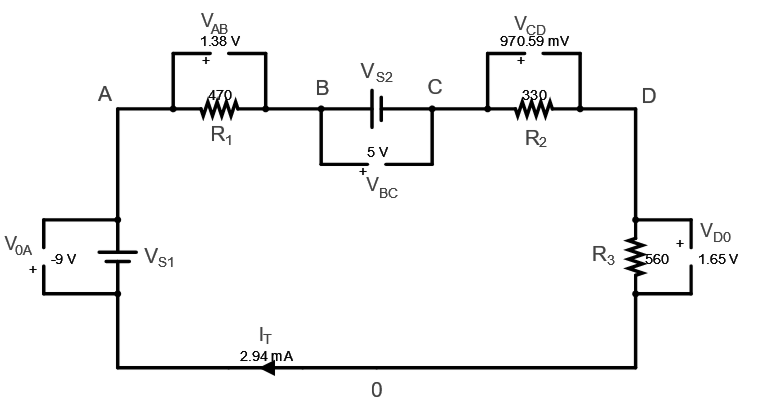
\includegraphics[width=.7\linewidth]{circ1}
    \caption{Simulation of the first circuit}
\end{figure}
%----------Circuit2
\subsection{Verification of Kirchhoff's Current Law}
In the next part we built the circuit according to this diagram:
%--------------------Diagram
\begin{minipage}{.7\textwidth}
    \begin{circuitikz}
        \draw (0,3) to [V=$V_{S1}$] (0,0)
        (0,3) to [R=$R_1$,*-*] (3,3) 
        to [R=$R_3$] (6,3) 
        to [V=$V_{S2}$,*-] (6,0) -- (0,0) 
        (3,0) to [R=$R_2$,*-] (3,3)
    {[anchor=south east](0,3) node {A}
    (3,3) node {B} 
    [anchor=north east](3,0) node {0}
    [anchor=south west](6,3) node {C}}; 
    \end{circuitikz}
\end{minipage}\raggedright
\begin{minipage}{.3\textwidth}
    \begin{tabular}{|c|c|c|}\hline
        Element & Value & Power Rat.\\\hline
        $V_{S1}$ & $\SI{9}{\volt}$ & $0$\\\hline
        $V_{S2}$ & $\SI{5}{\volt}$ & $0$\\\hline
        $R_1$ & $\SI{470}{\ohm}$ & $\SI{1/2}{\volt}$\\\hline
        $R_2$ & $\SI{330}{\ohm}$ & $\SI{1/2}{\volt}$\\\hline
        $R_3$ & $\SI{560}{\ohm}$ & $\SI{1/2}{\volt}$\\\hline
    \end{tabular}
\end{minipage}
\subsubsection{Calculations}
\justify
We can see that,in contrast with the previous circuit, now we have two meshes meaning that we have three different currents.In order to calculate the value of each current we must propose a direction of current for every mesh and assign polarity depending on the proposed direction.Then using Kirchhoff's Current Law in the left mesh:
\begin{gather*}
    -V_{S1}+VR_1+VR_2=0\\
    -9+470I_1+330(I_1-I_2)=0
\end{gather*}\\[-5ex]
\begin{equation}-800I_1-330I_2=9\label{eq:1}\end{equation}
for the right mesh:
\begin{gather*}
    VR_2+VR_3+V_{S2}=0\\
    330(I_2-I_1)+560I_2=0
\end{gather*}\\[-5ex]
\begin{equation}-330I_1+890I_2=-5\label{eq:2}\end{equation}
With \eqref{eq:1} and  \eqref{eq:2} we have the next linear system:
\[
    \begin{cases}
        -800I_1-330I_2=9\\
        -330I_1+890I_2=-5
    \end{cases}
\]
Expressing the system in matrices:
\[
    \begin{bmatrix}
        -800 & -330\\
        -330 & 890
    \end{bmatrix}
    \begin{bmatrix}
        I_1\\
        I_2
    \end{bmatrix}
    =
    \begin{bmatrix}
        9\\
        -5
    \end{bmatrix}
\]
Using Crammer's rule to solve the linear system:
\begin{gather*}
    \Delta=
    \begin{bmatrix}
        -800 & -330\\
        -330 & 890
    \end{bmatrix}
    =-800\times 890-(-330)\times(-330)\\
\Delta=603100\\
    \begin{bmatrix}
        -800 & -9\\
        -330 & 5
    \end{bmatrix}
    =-800\times 5-(-9)\times(-330)\\
    \Delta_1=6360\\
\Delta_2=
    \begin{bmatrix}
        -9 & -330\\
        5 & 890
    \end{bmatrix}
    =-9\times890-(-330)\times(5)\\
    \Delta_2=-1030
\end{gather*}
Finally:
\begin{gather*}
    I_1=\frac{\Delta_1}{\Delta}=\frac{6360}{603100}\si{\ampere}\qquad I_1=\SI{10.545}{\milli\ampere}\\[2ex]
    I_2=\frac{\Delta_2}{\Delta}=\frac{-1030}{603100}\si{\ampere}\qquad I_2=\SI{-1.708}{\milli\ampere}\\
\end{gather*}
Using Kirchhoff's Current Law in node B:
%redibujar circuito
%check!!!!!!!!!!!!
\begin{gather*}
I_1-I_2=I_3\\
I_3=\SI{10.545}{\milli\ampere}-(\SI{-1.708}{\milli\ampere})\\
I_3=\SI{12.253}{\milli\ampere}\\
\end{gather*}
The voltages for each segment are, for $V_{A0}$:
\begin{align*}
    V_{A0}&=V_{S1}\\
    V_{A0}&=\SI{9}{\volt}
\end{align*}
For $V_{AB}$:
\begin{align*}
    V_{AB}&=I_1R_1\\
    V_{AB}&=(\SI{10.545}{\milli\ampere})(\SI{470}{\ohm})\\
    V_{AB}&=\SI{4.956}{\volt}
\end{align*}
For $V_{B0}$:
\begin{align*}
    V_{B0}&=I_3R_1\\
    V_{B0}&=(\SI{10.545}{\milli\ampere})(\SI{330}{\ohm})\\
    V_{B0}&=\SI{4.043}{\volt}
\end{align*}
For $V_{BC}$:
\begin{align*}
    V_{BC}&=I_2R_1\\
    V_{BC}&=(\SI{10.545}{\milli\ampere})(\SI{470}{\ohm})\\
    V_{BC}&=\SI{-956.48}{\milli\volt}
\end{align*}
For $V_{C0}$:
\begin{align*}
    V_{C0}&=V_{S2}\\
    V_{C0}&=\SI{5}{\volt}
\end{align*}
Next, we calculate the power value for each segment of the circuit, in $P_{0A}$ we have:
\begin{align*}
    P_{0A}&=V_{0A}I_1\\
    P_{0A}&=(-\SI{9}{\volt})(\SI{10.545}{\milli\ampere})\\
    P_{0A}&=\SI{-94.905}{\milli\watt}
\end{align*}
In $P_{AB}$:
\begin{align*}
    P_{AB}&=V_{AB}I_1\\
    P_{AB}&=(\SI{4.956}{\volt})(\SI{10.545}{\milli\ampere})\\
    P_{AB}&=\SI{52.261}{\milli\watt}
\end{align*}
In $P_{B0}$:
\begin{align*}
    P_{B0}&=V_{B0}I_3\\
    P_{B0}&=(\SI{4.043}{\volt})(\SI{12.253}{\milli\ampere})\\
    P_{B0}&=\SI{49.539}{\milli\watt}
\end{align*}
In $P_{BC}$:
\begin{align*}
    P_{BC}&=V_{BC}I_2\\
    P_{BC}&=(\SI{-956.48}{\milli\volt})(\SI{-1.708}{\milli\ampere})\\
    P_{BC}&=\SI{1.634}{\milli\watt}
\end{align*}
In $P_{C0}$:
\begin{align*}
    P_{C0}&=V_{C0}I_2\\
    P_{C0}&=(\SI{5}{\volt})(\SI{-1.708}{\milli\ampere})\\
    P_{C0}&=\SI{-8.540}{\milli\watt}
\end{align*}
Finally, the sum of all powers is:
\begin{gather*}
    \sum\nolimits_{P}=P_{A0}+P_{AB}+P_{B0}+P_{BC}+P_{C0}\\
    \sum\nolimits_{P}=\SI{-94.905}{\milli\watt}+\SI{52.261}{\milli\watt}+\SI{49.539}{\milli\watt}+\SI{1.634}{\milli\watt}+\SI{-8.540}{\milli\watt}\\
    \sum\nolimits_{P}=\SI{-0.011}{\milli\watt}
\end{gather*}
\subsubsection{Measurements}
\begin{table}[H]
    \centering
    \begin{tabular}{|c|c|c|}\hline
        Measurements & Theoretical Value & Measured Value\\
        & (\si{\milli\ampere}) & (\si{\milli\ampere})\\\hline 
        Current $I_1$ (Left branch) & 10.545 & 10.560 \\\hline
        Current $I_2$ (Center branch) & 12.253 & 12.180 \\\hline
        Current $I_3$ (Right branch) & 1.708 & 1.175 \\\hline
    \end{tabular}
    \caption{Theoretical and measured current values}
    \label{table:2}
\end{table}
\begin{table}[H]
    \centering
    \resizebox{\textwidth}{!}{%
    \begin{tabular}{|c|c|c|c|c|c|c|}\hline
    Measurements & Theoretical & Measured & Theoretical & Measured &
    Absorb(A)/\\
        &  Value (\si{\volt}) &  Value (\si{\volt}) &  Power (\si{\milli\watt}) & Power (\si{\milli\watt}) & Supply(S)\\\hline
        Voltage $V_{0A}$ & -9.000 & -8.990 & -94.905 & -94.934  & S \\\hline
        Voltage $V_{AB}$ & 4.956 & 5.270 & 52.261 & 55.651 & A \\\hline
        Voltage $V_{B0}$ & 4.043 & 4.060 & 49.539 & 49.747 & A \\\hline
        Voltage $V_{BC}$ & \num{-956e-3} & \num{-888e-3}  & 1.634 & 1.673 & A \\\hline
        Voltage $V_{C0}$ & 5.000 & 5.020 & -8.540 & -8.750  & S \\\hline
      & $\sum_V=\SI{4.043}{\volt}$ & $\sum_V=\SI{6.24}{\volt}$ &
      $\sum_P=\SI{-0.011}{\milli\watt}$ & $\sum_P=\SI{3.387}{\milli\watt}$ & \\\hline
    \end{tabular}}
    \caption{Theoretical and measured voltage values}
    \label{table:3}
\end{table}
\subsubsection{Simulation}
\begin{figure}[H]
    \centering
    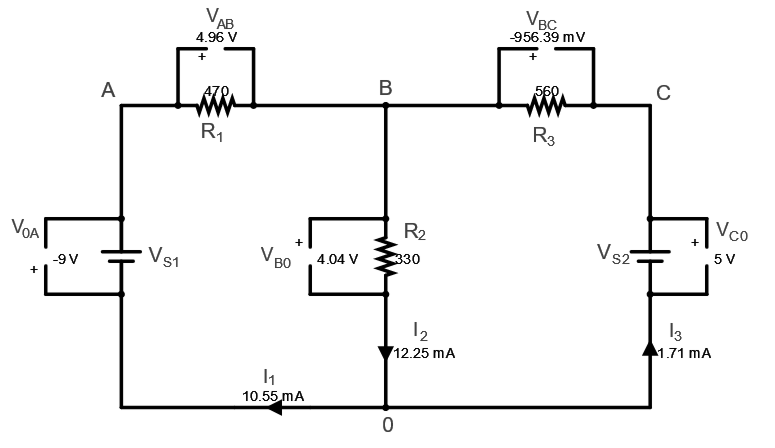
\includegraphics[width=.7\textwidth]{circ2}
    \caption{Simulation of the second circuit}
\end{figure}
\section{Questions}
\textbf{Define what is a node in an electrical circuit}:\\[0.5ex]
In an electrical circuit, a node is a point where two or more elements of circuits cross, a source of voltage or current, resistors, capacitors, inductors, etc.\\
\textbf{Define what is a electric circuit}:\\[0.5ex]
An electrical circuit is the interconnection of two or more components that contains a closed trajectory. These components can be resistors, sources, switches, etc.\\
\textbf{Express Kirchoff's Current Law in mathematical terms}:\\[0.5ex]
\[\sum_{k=1}^n I_k=0\]
where $n$ is the total number of branches with currents flowing towards or away from the node.\\
\textbf{Define what is a closed trajectory in an electrical circuit}:\\[0.5ex]
A circuit is closed if the circle is complete, if all the currents have a path back to where they started.\\
\textbf{Define what is voltage drop}:\\[0.5ex]
Voltage drop describes how the energy supplied by a voltage source is reduced as electric current moves through the passive elements of an electrical circuit. The voltage drop across the internal resistance of the source, across conductors, contacts, and connectors is undesirable because some of the energy supplied is lost.\\
\section{Conclusions}
\justify
{\large\textbf{Sabrina}:}\\[0.5ex]
In reality, we won’t encounter simple, reducible circuits all the time. We need Kirchhoff’s laws to analyze thoroughly and efficiently circuits that can't be reduced, which may have loops (also called mesh), several power sources or won't be connected in parallel or series at all. It is one of the basic concepts to understand electric circuits and their properties. Although the demonstration of these laws may go beyond our actual understanding of circuits, it was possible for the team to do the laboratory practice without too much difficulty to apply said laws and note how everything works in the physical circuit (approximately) like it would do theoretically.\\[2ex]
{\large\textbf{Salvador}:}\\[0.5ex]
For an Engineer it’s crucial know how an electrical circuit works. In this practice we use Kirchhoff’s law of current to measure the current in the first circuit, because we knew that the current was the same throughout the circuit\\[2ex]
{\large\textbf{Sebastián}:}\\[0.5ex]
In this experiment we experienced the different behavior of voltage in current between two different types of circuits, one  single loop and the other with two meshes, concluding that, in the case of the first, the current value was the same along the whole loop but the voltage and the power values varied between each branch,in contrast, the other circuit had three different currents flowing between the two meshes and therefore different voltage and power values between branches. Summing the voltage and power measurements in the first experiment, we could see that the total approximates to zero, proving Kirchhoff's Voltage Law. In the case of the second experiment the whole sum of voltage values is not even near zero and this is because we are summing everything as if it were a single loop, in reality, we have two meshes and the individual sum of the voltages in each mesh with the right sign according to the current of the loop, yields nearly zero, therefore proving Kirchhoff's Voltage Law, however, in the case of power values, the total sum is close to zero.
\\[2ex]
\end{document}
